% Prof. Dr. Ausberto S. Castro Vera
% UENF - CCT - LCMAT - Curso de Ci\^{e}ncia da Computa\c{c}\~{a}o
% Campos, RJ,  2023
% Disciplina: Paradigmas de Linguagens de Programa\c{c}\~{a}o
%


\chapter{ Aplica\c{c}\~{o}es da Linguagem R}
	Neste capítulo vamos, a partir do que aprendemos nos capítulos anteriores, colocar à teste a Linguagem R quanto as suas aplicações.\par Veremos, na prática, como os conceitos básicos conversam com as áreas de aplicação, desde operações básicas até aplicações com banco de dados. Praticaremos com exemplos, códigos completos com resultados e principalmente, a descrição desses programas, como funcionam e suas características. Vamos à prática.
    %%%--------------------------------------------------------------------
    \section{Opera\c{c}\~{o}es b\'{a}sicas}
    %%%--------------------------------------------------------------------    
    Em \cite{Lander2017} vemos que na programação é melhor diminuir a redundância sempre que possível, e as funções são uma ótima maneira de fazer isso.\par Nessa seção vamos analisar um código básico para calcular o volume de um cilindro de uma forma totalmente interativa. Utilizaremos as ferramentas detalhadas no capítulo anterior.
     \begin{figure}[H]
     	\centering
     	\caption{}
     	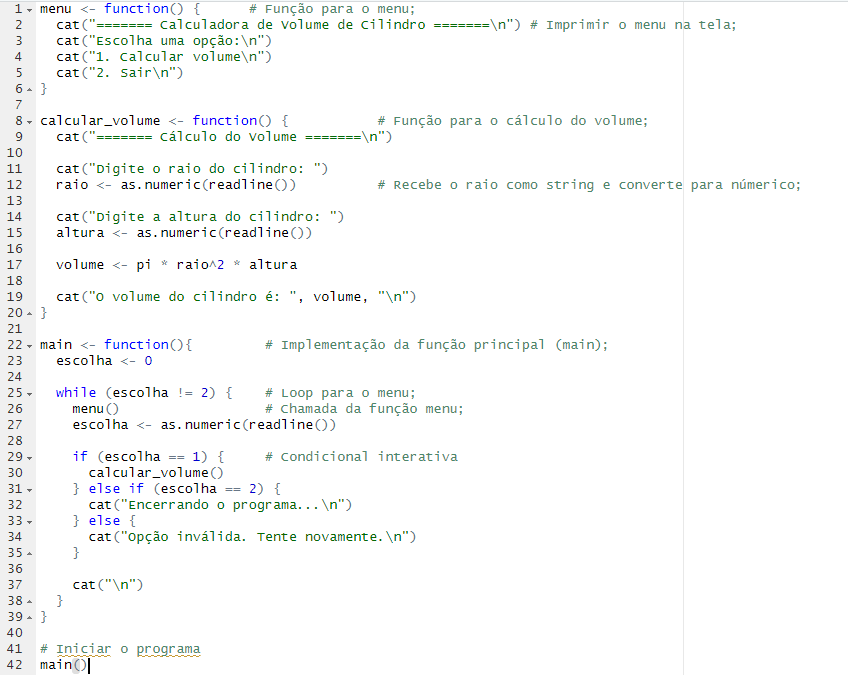
\includegraphics[width=1.0\linewidth]{Prints/screenshot018}
     	\label{fig:screenshot018}
     	{\tiny \sf Fonte: O autor deste trabalho }
     \end{figure}
      Aprenderemos na prática a utilização das funções. Assim como na aplicação, a descrição será divida pelas funções.
      \subsection{Função menu}
      No começo do código, declaramos e implementamos a função para o menu interativo, sendo o procedimento mais simples do programa, consiste apenas na impressão das quatro linhas de menu na tela, dando ênfase ás duas opções dadas ao usuário. \par Essa impressão funciona com a função nativa 'cat()' que serve para imprimir mensagens concatenadas. Também poderia ter sido usado a função 'print ()', nesse caso.
      \subsection{Função calcular\_volume}
      Após o título do calculo de volume, impresso por 'cat()', é pedido ao usuário o raio do cilindro. O R possui algumas formas de entrada de dados, como 'scan()' que armazena os valores em vetores de acordo com o tipo de dado detectado. Nesse caso utilizaremos a função 'readline()' que recebe qualquer tipo de valor de entrada como uma string. Pode-se notar que a variável 'raio' não recebe diretamente o dado da entrada recebido por 'readline()', como se fosse "raio <- readline()". Esse fato se dá por conta do que foi dito acima, essa função de entrada recebe qualquer coisa como string, sendo assim, necessitaremos de uma outra função pra nos auxiliar nessa conversão de string para númerico. Intuitiva, utilizaremos a função 'as.numeric ()' passando como argumento o que for recebido na função 'readline ()'. Sendo assim, a variável 'raio' receberá o que for retornado pela função 'as.numeric()', que por sua vez, recebe o que for retornado pela função 'readline ()'.\par É feita a exata mesma operação para pedir e receber o valor da altura do cilindro.\par Depois de recebidas todas as informações necessárias, é declarada a variável 'volume' que recebe o resultado da conta "pi*raio²*altura".\par Por fim, a função imprime o valor desse volume. Uma outra opção seria retornar o valor para fora da função e então imprimi-la, mas foi escolhido a imporessão dentro da função.
      \subsection{Função main}
      Em R, diferentemente de outras linguagens, não há a necessidade de uma função main para iniciar um programa. As funções funcionam independentemente. Por conta de organização e estruturação, chamaremos de main a função onde acontecerá de fato o programa como uma unidade.\par Para começar, declaramos a variável 'escolha' como zero, essa sendo a definição do usuário no menu. Em sequência, entraremos no laço while que tem como condição a variável 'escolha' ser diferente de 2, veremos como funciona esse laço. Assim que entramos na repetição, é chamada a função 'menu()' que imprime o menu indicando o que o usuário deve fazer, entretanto, a resposta não é recebida dentro dessa função, ela unicamente imprime na tela, sendo assim, temos, em seguida, o recebimento da opção do usuário, que é guardada na variável 'escolha'. Esse recebimento funciona com base na função 'as.numeric()' vista anteriormente.\par Após isso, entramos em uma condicional if-else (ainda dentro do while) que tem como condição o valor da variável 'escolha' ser 1, 2 ou outra, cada uma dessas opções tem linhas a se seguir.\par A primeira, significando que o usuário escolheu calcular o volume do cilindro, chamaria a função 'calcula\_volume' que, como dito, imprime o resultado dentro dela própria, sem a necessidade de retornar o valor calculado em outra variável para ser impressa.\par A segunda opção, significando que o usuário escolheu sair do programa, mostra na tela uma mensagem encerrando o programa.\par Por fim, a terceira opção, caso o usuário digite algum valor que não sejam os dois válidos, é impressa uma mensagem avisando que a opção é inválida.\par Como dito, em R as funções funcionam independentemente, então por mais que em outras linguagens, a implementação da função main ja seja a execução dela, nesse caso, o main foi apenas o nome dado, não existe de fato uma função principal. Sendo assim, é necessário que no fim do programa, essa função "principal" seja chamada e passe a executar.
	  Veremos abaixo a execução e o resultado desse programa.
	  \begin{figure}[H]
		  \centering
		  \caption{}
		  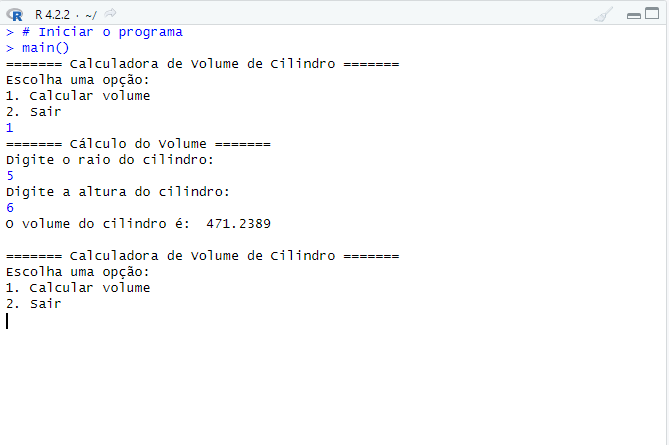
\includegraphics[width=1.0\linewidth]{Prints/screenshot019}
		  \label{fig:screenshot019}
		  {\tiny \sf Fonte: O autor deste trabalho }
	  \end{figure}
	Essa foi uma aplicação básica de um programa para calcular o volume de um cilindro de forma interativa. Vimos sobre funções em geral e laços básicos. Continuaremos vendo outras aplicações dessa linguagem.

    %%%--------------------------------------------------------------------
    \section{Programas gr\'{a}ficos}
    %%%--------------------------------------------------------------------    
    Como dito anteriormente, a linguagem R é bastante utilizada para representar problemas e programas gráficos, e para fazer isso, recebe o auxílio de diversos pacotes que disponibilizam variadas funções com esse objetivo. Nessa seção utilizaremos o pacote, ja citado, 'ggplot2'. Tudo referido à esse pacote teve como base o \cite{Wickham2016} e o index oficial do pacote \url{https://ggplot2.tidyverse.org/reference/index.html}.
    \par Analisaremos um programa simples que recebe três equações e gera um gráfico pra cada uma delas.
    \begin{figure}[H]
    	\centering
    	\caption{}
    	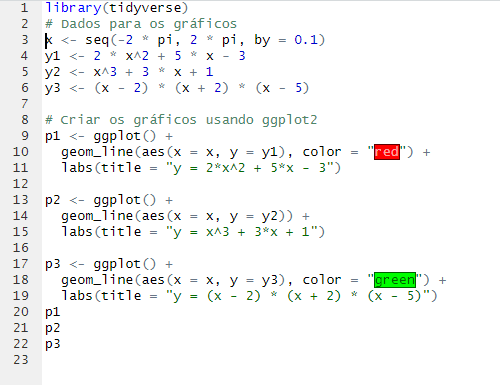
\includegraphics[width=1.0\linewidth]{Prints/screenshot020}
    	\label{fig:screenshot020}
    	{\tiny \sf Fonte: O autor deste trabalho }
    \end{figure}
	
	\subsection{Dados para os gráficos}
	Primeiramente, precisamos carregar a biblioteca que usaremos. Nesse caso, como visto no \cite{Wickham2016}, utilizaremos a 'tidyverse' que nada mais é do que uma coleção de pacotes em R. Nesse programa, será usado o 'ggplot2', que faz parte dessa coleção.\par As próximas quatro linhas são apenas os valores das variáveis que serão utilizadas nos gráficos. Cada Y recebendo uma equação diferente em função de X.
    
    \subsection{Criando os gráficos}
    A variável 'p1' recebe o gráfico de y1 através da função ''ggplot()'. Essa função cria um sistema de coordenadas em que é possível adicionar camadas. Pode-se rodar o programa a partir dessa linha, visto que o gráfico foi criado, mas apenas mostraria um gráfico vazio, ou seja, precisamos adicionar camadas à ele.\par Para completar o gráfico vamos usar a função 'geom\_line', que adiciona uma camada de linha para o nosso gráfico (o pacote disponibiliza diversas formas de gráficos, mas utilizaremos de linha). Cada função no ggplot2 possui um mapeamento de argumentos que definem como as variáveis serão mapeadas em um gráfico. Podemos ver esse mapeamento com o 'aes()' que tem como argumentos x e y, que especificam quais variáveis se devem mapear nos eixos x e y. Nesse caso, a variável X foi a mesma para os três gráficos, e o Y foi variando entre as equações definidas. Por fim, fora do mapeamento, é definida a cor da linha manualmente com o "color = red" no 'p1' e "color = green" no 'p3'. O 'p2' não foi definida a cor e, por isso, foi estabelecido como preto.\par Depois de adicionadas as camadas do gráfico, foi utilizada a função 'labs()' para adicionar o título. Essa função é utilizada para adicionar rótulos, em geral, ao gráfico. Nesse caso, adicionamos apenas o título, que é a equação que o gráfico representa.
    \begin{figure}[H]
    	\centering
    	\caption{Gráfico p2:}
    	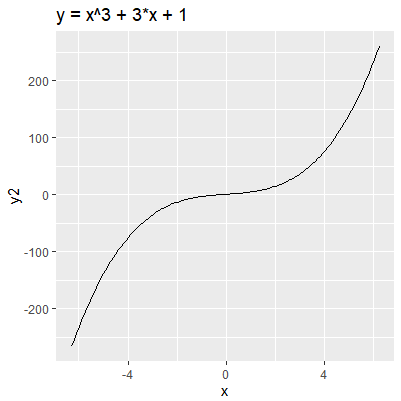
\includegraphics[width=1.0\linewidth]{Prints/screenshot021}
    	\label{fig:screenshot021}
    	{\tiny \sf Fonte: O autor deste trabalho }
    \end{figure}
    Na Figura acima, é mostrado o gráfico da equação 'p2'. Como dito acima, por não ter recebido mapeamento de cor, a linha foi padronizada preta.
    %%%--------------------------------------------------------------------
    \section{Programas com Objetos}
    %%%--------------------------------------------------------------------    
    Aprenderemos agora um pouco mais sobre a ja comentada programação orientada a objetos. Como vimos, R possui três sistemas diferentes de orientação a objetos (s3, s4 e RC), e cada uma tem suas próprias características. Vamos então analisar uma aplicação partindo do princípio da Reference Class, que é o sistema mais completo dos três.
    \begin{figure}[H]
    	\centering
    	\caption{Reference Class}
    	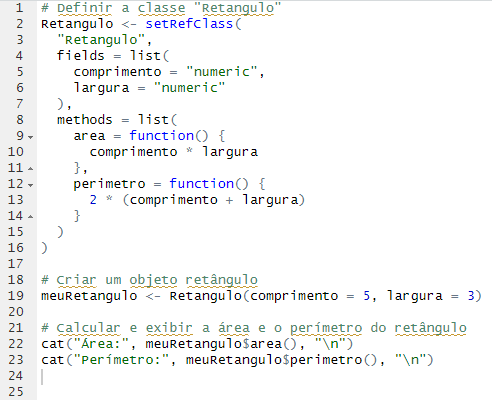
\includegraphics[width=1.0\linewidth]{Prints/screenshot022}
    	\label{fig:screenshot022}
    	{\tiny \sf Fonte: O autor deste trabalho }
    \end{figure}
    Logo no começo, definimos uma nova classe 'Retangulo' com a função "setRefclass" que é exclusiva para criação de classes no Reference Class, assim iniciando nosso projeto nesse sistema.\par Em seguida, estabelecemos seus atributos utilizando o 'fields', que é a forma utilizada pelo RC, e criamos essa lista de atributos que consiste no comprimento e na largura, ambos númericos. Por fim, foram definidos os métodos da classe, esses sendo 'area', que é uma função que multiplica o comprimento pela largura, e 'perimetro' que é uma função que multiplica por 2 a soma dos dois atributos.\par Seguindo então,  criamos um novo objeto "meuRetangulo" pertencente à essa classe atribuindo a ele a passagem da classe com os atributos comprimento e largura como 5 e 3, respectivamente.\par Por fim, imprimimos a área do objeto "meuRetangulo" ao chamar o método área com o "meuRetangulo\$area". A mesma coisa é feita com o perímetro.
    
    %%%--------------------------------------------------------------------
    \section{O algoritmo Quicksort - Implementa\c{c}\~{a}o}
    %%%--------------------------------------------------------------------    
    Caminharemos sobre um algoritmo importante de ordenação chamado de Quicksort. Trabalhando com base em "dividir e conquistar", esse algoritmo define um pivô onde todos os números à sua esquerda são menores do que ele e todos à sua direita são maiores que ele, então recursivamente faz o mesmo procedimento com sua partes divididas. Entenderemos melhor na prática. 
   \begin{figure}[H]
   		\centering
   		\caption{Quicksort}
   		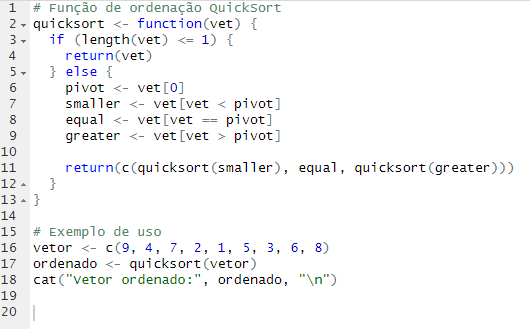
\includegraphics[width=1.0\linewidth]{Prints/screenshot023}
   		\label{fig:screenshot023}
   		{\tiny \sf Fonte: O autor deste trabalho }
   \end{figure}
   \subsection{Chamada da função}
   Por organização, vamos, primeiramente, analisar a parte de baixo do código. Primeiramente, um vetor desordenado é declarado na variável 'vetor'. Então é declarada a variável 'ordenado', que recebe o que é retornado da função "quicksort(vetor)" (analisaremos ela em seguida). Por fim, é impresso na tela essa variável 'ordenado'. Já veremos o que ela recebe.
   \subsection{Quicksort}
   Agora vamos discorrer sobre a função de ordenação. Primeiro, percebamos que ela recebe como argumento o vetor desordenado que foi declarado embaixo, então entra num 'If-else' que tem como condição o 'length(vet) <= 1', ou seja, se o tamanho do vetor for menor ou igual a 1, ele entra na condição de retornar o vetor como está (essa condição que dará fim à nossa recursão, veremos à frente), caso não satisfaça a condição e o vetor seja maior que 1, a função passa a declarar quatro variáveis: um pivô que recebe o valor que está na posição 0 do vetor, um smaller que recebe um vetor com todos os valores menores que o valor de pivô, um equal que recebe um vetor com todos os números iguais ao valor de pivô, e um greater que recebe um vetor com todos os números maiores. Ou seja, agora ja temos a primeira divisão: um vetor á esquerda com todos os valores menores que o pivô, o meio e um vetor à direita com todos os maiores.\par Agora é que a magia acontece. Depois de criar esses três dispositivos, a função retorna três coisas: o valor recebido de uma nova função quicksort, mas dessa vez passando o vetor recebido por smaller como argumento, o equal e o valor recebido de mais uma nova função quicksort, mas dessa vez passando o vetor recebido por greater como argumento. Assim acontecem mais duas ordenações paralelas, a do vetor smaller e do vetor greater, e cada uma dessas gera mais duas, e mais duas... Assim vai até cada uma se resolver totalmente e os vetores passados sejam apenas um valor, fazendo o que foi dito acima, saíriamos do if, retornando a concatenação de cada uma dessas ordenações com a função 'c()' para a variável 'ordenado', que é impresso logo após. 
   \begin{figure}[H]
   	\centering
   	\caption{Quicksort}
   	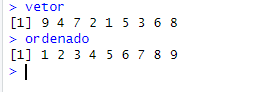
\includegraphics[width=1.0\linewidth]{Prints/screenshot024}
   	\label{fig:screenshot024}
   	{\tiny \sf Fonte: O autor deste trabalho }
   \end{figure}
   Por mais que um pouco complexa, essa forma de ordenação é bastante eficiente.
    
    %%%--------------------------------------------------------------------
    \section{Aplica\c{c}\~{o}es com Banco de Dados}
    %%%--------------------------------------------------------------------    
    Por fim, veremos a aplicação da R com os bancos de dados. Analisaremos um código onde utilizaremos o banco de dados disponibilizado no 'SQLite', criaremos uma tabela básica de dados e a imprimiremos, recebendo essas informações. Vamos analisar.
    \begin{figure}[H]
    	\centering
    	\caption{Quicksort}
    	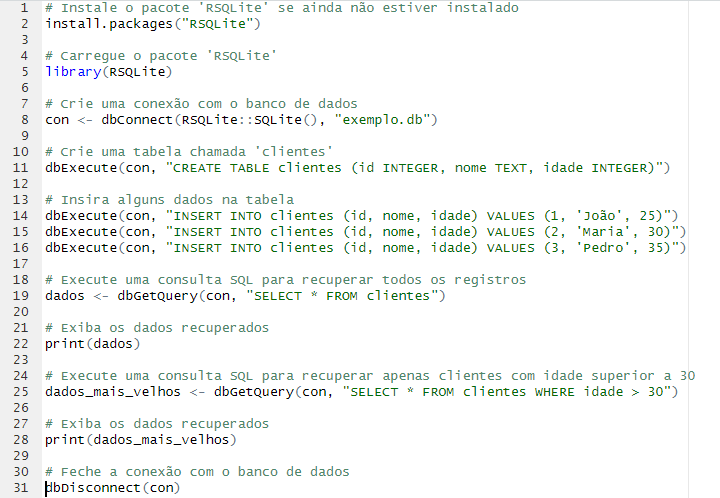
\includegraphics[width=1.0\linewidth]{Prints/screenshot025}
    	\label{fig:screenshot025}
    	{\tiny \sf Fonte: O autor deste trabalho }
    \end{figure}
    \subsection{Conectando e criando o banco de dados}
    Primeiramente, precisaremos instalar o o pacote 'RSQLite', que é um pacote que permite a conexão e interação com bancos de dados SQLite usando o R. Em seguida, carregamos esse pacote no nosso programa. Então estabelecemos uma conexão com o banco de dados. A função 'dbConnect()' é usada para criar essa conexão, e o argumento RSQLite::SQLite() especifica o driver SQLite para a conexão. O segundo argumento, "exemplo.db", é o nome do arquivo do banco de dados SQLite que será criado. Nesse caso, o arquivo será chamado "exemplo.db". \par Por fim, depois de termos instalado o pacote e conectado ao banco de dados, usaremos a função 'dbExecute()' para criar uma nova tabela no banco de dados. A função recebe dois argumentos: 'con' representa a conexão com o banco de dados e a criação da tabela clientes com o comando 'CREATE TABLE <nome da tabela>', recebendo então três elementos, 'id' e 'idade' sendo inteiros e 'nome' sendo texto.
    \subsection{Inserindo dados e os exibindo}
    Após criada a tabela, utilizaremos novamente a função 'dbExecute()', dessa vez recebendo, além do argumento con, argumento com o comando 'INSERT INTO <tabela>' para inserir dados na tabela com o comando 'VALUES <valores inseridos>', inserindo então o id, o nome e a idade de cada elemento da tabela.\par Após inseridas as informações, a variável 'dados' recebe o retornado pela função 'dbGetQuery()'. Essa função é usada para executar uma consulta no banco de dados e recuperar os resultados. A consulta SQL especificada é "SELECT * FROM clientes", que retorna todos os registros da tabela "clientes". Então imprime na tela essa variável 'dados'.\par Cria uma outra variável 'dados\_mais\_velhos' que recebe o retornado por outra função 'dbGetQuery()'. Dessa vez é executada para recuperar apenas os clientes com idade superior a 30. A consulta é "SELECT * FROM clientes WHERE idade > 30". Imprime esses dados mais velhos e para terminar, desconecta do banco de dados.
    
